\documentclass[../main.tex]{subfiles}
\begin{document}

\chapter{Dokumentacja deweloperska aplikacji}

\section{Stos technologiczny}
W sekcji \ref{sec:application_technology_choices_theory} opisane i uargumentowane zostały główne wybory technologii do stworzenia aplikacji dla części praktycznej niniejszego opracowania. W tej części uszczegółowiono wybór istotniejszych (według kryterium funkcjonalności) rozwiązań wraz z krótką charakterystyką, za co są odpowiedzialne w stworzonej aplikacji.

\subsection{Aplikacja mobilna}

\begin{itemize}
	\item react-native -- framework odpowiedzialny za tworzenie komponentów aplikacji takich jak poszczególne widoki (widok okna czatu, lista czatów (\textit{chat rooms}, widok ustawień), sam framework umożliwia lub ułatwia też korzystanie z szeregu bibliotek rozwijanych przez Meta Open Source\cite{meta_opensource} oraz społeczność niezależnych twórców.
	\item react-native-async-storage -- biblioteka daje dostęp do pamięci zachowawczej aplikacji, dzięki czemu możliwe jest przechowywanie konfiguracji aplikacji i odtwarzanie jej po jej uruchomieniu. Pamięć ta jest nieszyfrowana, dlatego dane wrażliwe, takie jak klucze RSA użytkownika i hasło logowania przechowywane są w inny sposób.
	\item react-native-gifted-chat -- biblioteka implementująca widok i funkcjonalności czatu, dzięki której dodając własną logikę odbierania wiadomości z serwera czy wczytywania archiwalnych wiadomości z pamięci można w prosty sposób wyświetlać otrzymane i wysłane wiadomości oraz tworzyć nowe.
	\item react-native-mmkv -- biblioteka umożliwiająca korzystanie z bardzo szybkiej bazy danych MMKV typu klucz-wartość na urządzenia mobilne. Baza danych daje możliwość szyfrowania jej zawartości, dlatego została wykorzystana do przechowywania poufnych danych użytkownika, takich jak login i hasło logowania.
	\item react-native-qrcode-svg -- biblioteka do generowania kodów QR wykorzystana do tworzenia obrazków z kodami zawierającymi klucz publiczny użytkownika, które można przesyłać osobom, z którymi chce się komunikować.
	\item react-native-rsa-native -- biblioteka implementująca generowanie kluczy RSA i funkcjonalności z nimi związane (szyfrowanie, deszyfrowanie, podpisywanie dokumentów). Biblioteka została zaimplementowana w sposób natywny (z użyciem języków Java, Swift i Objective C) i jest bardzo wydajna, co przekłada się na krótki czas generowania kluczy.
	\item react-navigation -- biblioteka udostępniająca komponenty umożliwiające użytkownikowi nawigację, czyli przechodzenia między widokami. Są to elementy takie jak dolny pasek nawigacji z zakładkami.
	\item expo -- jest to platforma, w skład której wchodzi zestaw bibliotek ułatwiających tworzenie aplikacji w oparciu o framework React Native. Sama platforma zapewnia też narzędzia, zarówno lokalne (expo-cli) jak i chmurowe (\textit{Expo Application Services}, EAS) wspomagające proces budowania i debugowania aplikacji, publikowania aplikacji do sklepów Apple App Store i Google Play Store oraz zarządzania dependencjami czy migracji do kolejnych wersji SDK platformy. W skład tej platformy wchodzą liczne biblioteki ułatwiające pracę z różnymi komponentami systemu operacyjnego urządzenia mobilnego (np. zarządzanie uprawnieniami, dostęp do kamery, dostęp do systemu plików).
    \item expo-crypto -- biblioteka oferująca różne funkcje kryptograficzne, wykorzystana została do generowania kryptograficznie bezpiecznych (o wysokim poziomie pseudo losowości) ciągów bitów wykorzystywanych jako klucze sesji.
	\item expo-file-system -- biblioteka zapewniająca dostęp do systemu plików urządzenia. Istotnym ograniczeniem jest tu dostęp jedynie do plików w ramach pamięci przydzielonej danej aplikacji, nie ma możliwości uzyskania dostępu do plików użytkownika znajdujących się poza nią. Jednak na potrzeby stworzonej aplikacji było to wystarczające. Biblioteka została wykorzystana do zapisu i odczytu plików tekstowych oraz kodów QR zawierających klucze RSA.
	\item expo-media-library -- biblioteka zapewniająca dostęp do albumów zdjęć i tzw. rolki aparatu w telefonie. Została wykorzystana do zapisania w nich wygenerowanych kodów QR w formie obrazków rastrowych.
	\item expo-barcode-scanner -- biblioteka implementująca funkcjonalność skanera kodów QR, dzięki niej deweloper w prosty sposób może uruchamiać aparat urządzenia z odpowiednią konfiguracją oraz zarządzać rezultatami skanowania.
	\item expo-permissions -- biblioteka pozwalająca w prosty sposób zarządzać uprawnieniami aplikacji do dostępu do pewnych funkcji i zasobów urządzenia, takich jak dostęp do systemu plików, lokalizacji czy dostęp do aparatu.
	\item expo-sqlite -- biblioteka pozwalająca na dostęp do bazy danych SQLite. Baza ta jest wykorzystywana na urządzeniu do przechowywania historii wiadomości oraz danych o kontaktach użytkownika.
	\item expo-sharing -- biblioteka umożliwiająca użytkownikowi przesłanie treści różnymi kanałami komunikacji. Została wykorzystana, aby dać klientowi możliwość przesłania kodu QR lub pliku tekstowego z kluczem publicznym. Użytkownik w interfejsie graficznym sam wybiera poprzez którą z dostępnych na jego urządzeniu aplikacji udostępnić te treści.
    \item noble-hashes - biblioteka implementująca wiele popularnych funkcji skrótu, wykorzystano zawartą w niej implementację funkcji hashującej BLAKE3.
	\item zustand -- biblioteka do zarządzania stanem aplikacji (pamięcią podręczną). Wykorzystana została do przechowywania konfiguracji niezachowawczej programu oraz usprawnień podnoszących wydajność aplikacji, takich jak przechowywanie kontekstu potrzebnego do pewnych działań (np. klucze sesji wykorzystywane każdorazowo przy szyfrowaniu wysyłanych lub odszyfrowywaniu metodą SDEx otrzymywanych wiadomości).
	\item socket.io-client -- biblioteka implementująca protokół WebSocket. Umożliwia ona m.in. nawiązywanie połączenia z serwerem, definiowanie emiterów wiadomości do serwera oraz modułów odpowiedzialnych za odbieranie wiadomości z niego przychodzących.
\end{itemize}

\subsection{Aplikacja serwerowa}

\begin{itemize}
	\item fastapi -- asynchroniczny framework webowy wykorzystany do stworzenia API umożliwiającego funkcjonowanie aplikacji mobilnej.
	\item fastapi-socketio -- biblioteka służąca do integracji socket.io (implementacji protokołu WebSocket) z frameworkiem FastAPI
	\item uvicorn -- implementacja serwera webowego w Pythonie. Wspiera HTTP/1.1, HTTP/2 i WebSocket.
	\item pydantic -- biblioteka służąca do weryfikowania poprawności danych w oparciu o typowanie w Pythonie (tzw. \textit{type hints}). W oparciu o tę bibliotekę zbudowany został także framework FastAPI. Biblioteka wykorzystywana jest do modelowania struktur danych znajdujących się w bazie danych serwera.
	\item rsa -- biblioteka implementująca RSA w języku Python. Oferuje możliwość generowania pary kluczy, szyfrowania, deszyfrowania, a także podpisywania i weryfikacji podpisów.
\end{itemize}

\section{Instalacja i uruchomienie aplikacji}

\subsection{Instrukcje dla aplikacji serwerowej}

Do obsługi i utrzymania aplikacji serwerowej przygotowany został plik Makefile zawierający przygotowane komendy (tzw. \textit{targets}) do uruchomienia aplikacji, testów, lintowania i formatowania kodu oraz uaktualniania bibliotek do nowszych wersji zgodnych z użytą wersją języka Python oraz zgodnych między sobą (rozwiązaniem kwestii zgodności, czyli zarządzaniem dependencjami zajmuje się narzędzie Poetry \cite{poetry}). Wykorzystanie Makefile wiąże się z koniecznością posiadania zainstalowanego programu make (dostępnego na większości popularnych systemów operacyjnych), można jednak wykonać wyżej wymienione czynności bez niego kopiując komendy przypisane do wybranego targetu. Przykładowo aby zainstalować i uruchomić aplikację należy wywołać w wybranej przez siebie powłoce (będąc w katalogu głównym aplikacji serwerowej

\code{kod_aplikacji/SDEx-encrypted-communicator/server}):

\begin{lstlisting}[style=BashInputStyle]
    $ make install
    $ make run
\end{lstlisting}
lub
\begin{lstlisting}[style=BashInputStyle]
    $ poetry install
    $ poetry run python sdex_server/main.py
\end{lstlisting}

pełna lista komend znajduje się w pliku:

\code{kod_aplikacji/SDEx-encrypted-communicator/server/Makefile}


\subsection{Instrukcje dla aplikacji mobilnej}

Aplikację mobilną można zainstalować wgrywając plik \code{.apk} znajdujący się w archiwum dołączonym do niniejszego opracowania.

Aby zbudować  ten plik na bazie napisanego kodu należy przygotować środowisko (zainstalować npm, Expo, założyć konto na \url{https://expo.dev/} oraz zalogować się w powłoce przy pomocy swoich danych do konta komendą \code{eas login}, a następnie przejść do katalogu głównego aplikacji mobilnej:

\code{kod_aplikacji/SDEx-encrypted-communicator/server/sdex-encrypted-communicator} i wywołać komendę:

\begin{lstlisting}[style=BashInputStyle]
    $ eas build -p android --profile production
\end{lstlisting}

następnie przejść na stronę: \url{https://expo.dev/accounts/<login>} (dostępną po zalogowaniu) i pobrać utworzony przez usługę Expo EAS plik instalacyjny \code{.apk} (Rysunek \ref{fig:builds-list} i \ref{fig:download-build})

\begin{figure}[H]
	\centering
	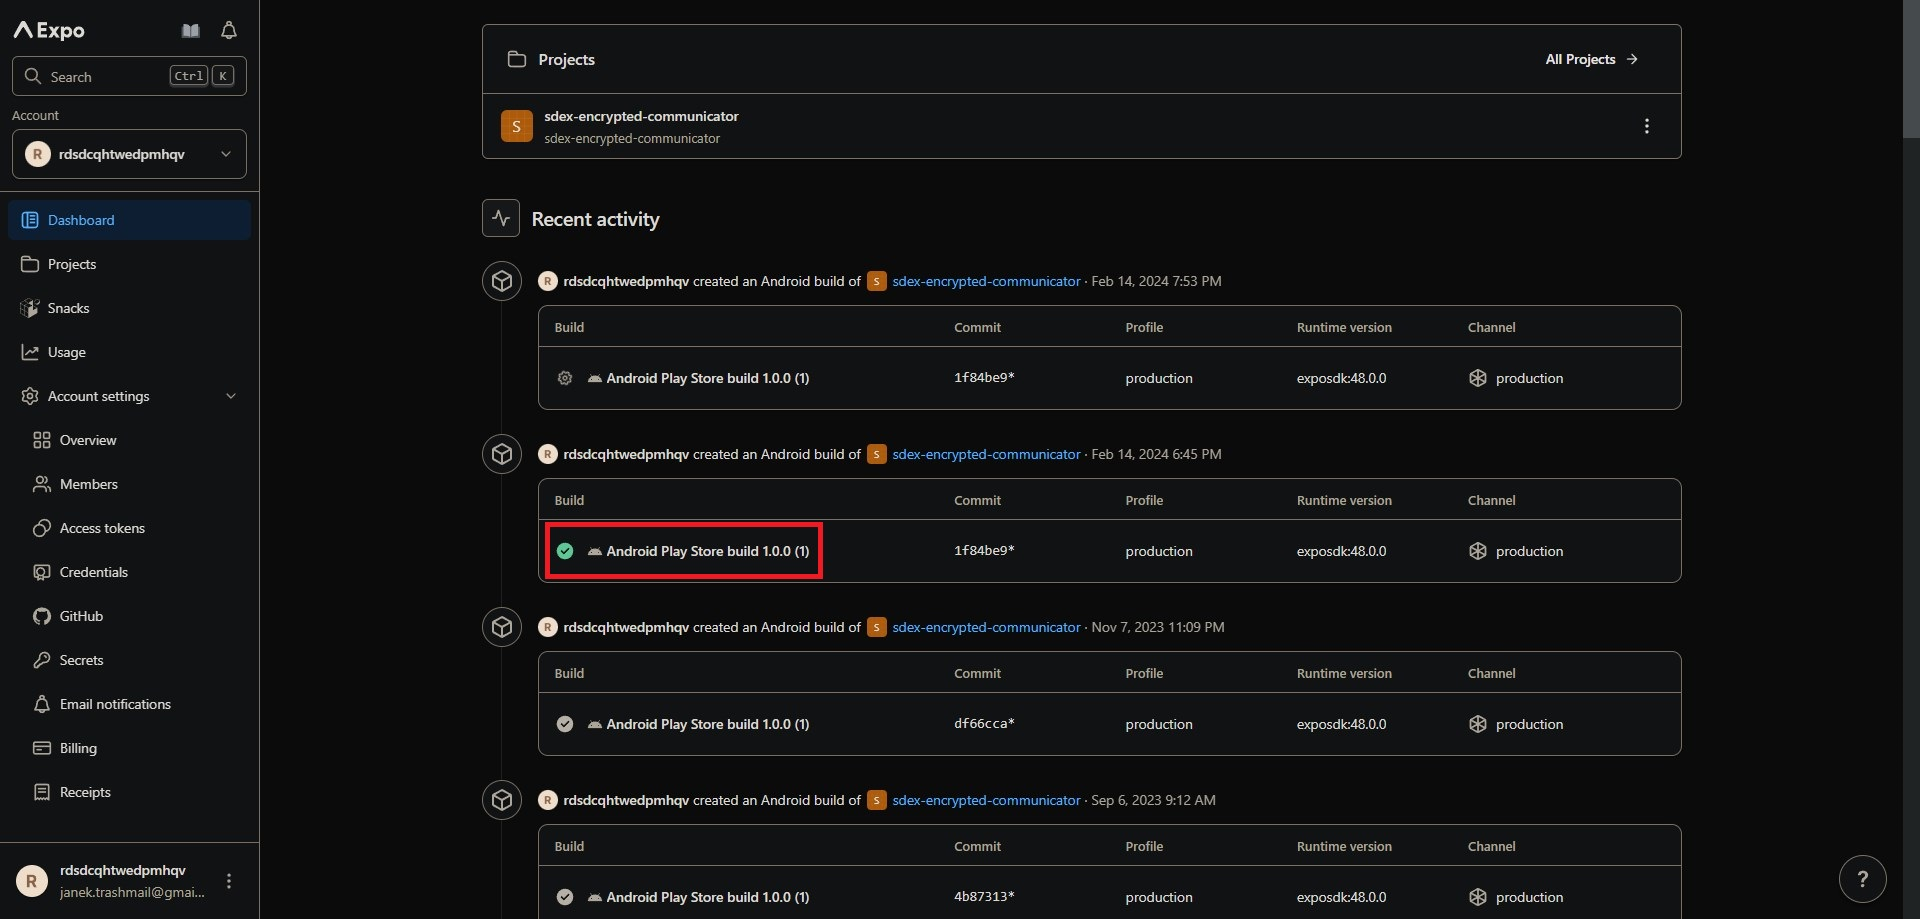
\includegraphics[scale=0.31]{download-apk-1.jpg}
	\caption{Widok strony z dostępnymi zbudowanymi wersjami aplikacji}
	\source{opracowanie własne}
	\label{fig:builds-list}
\end{figure}

\begin{figure}[H]
	\centering
	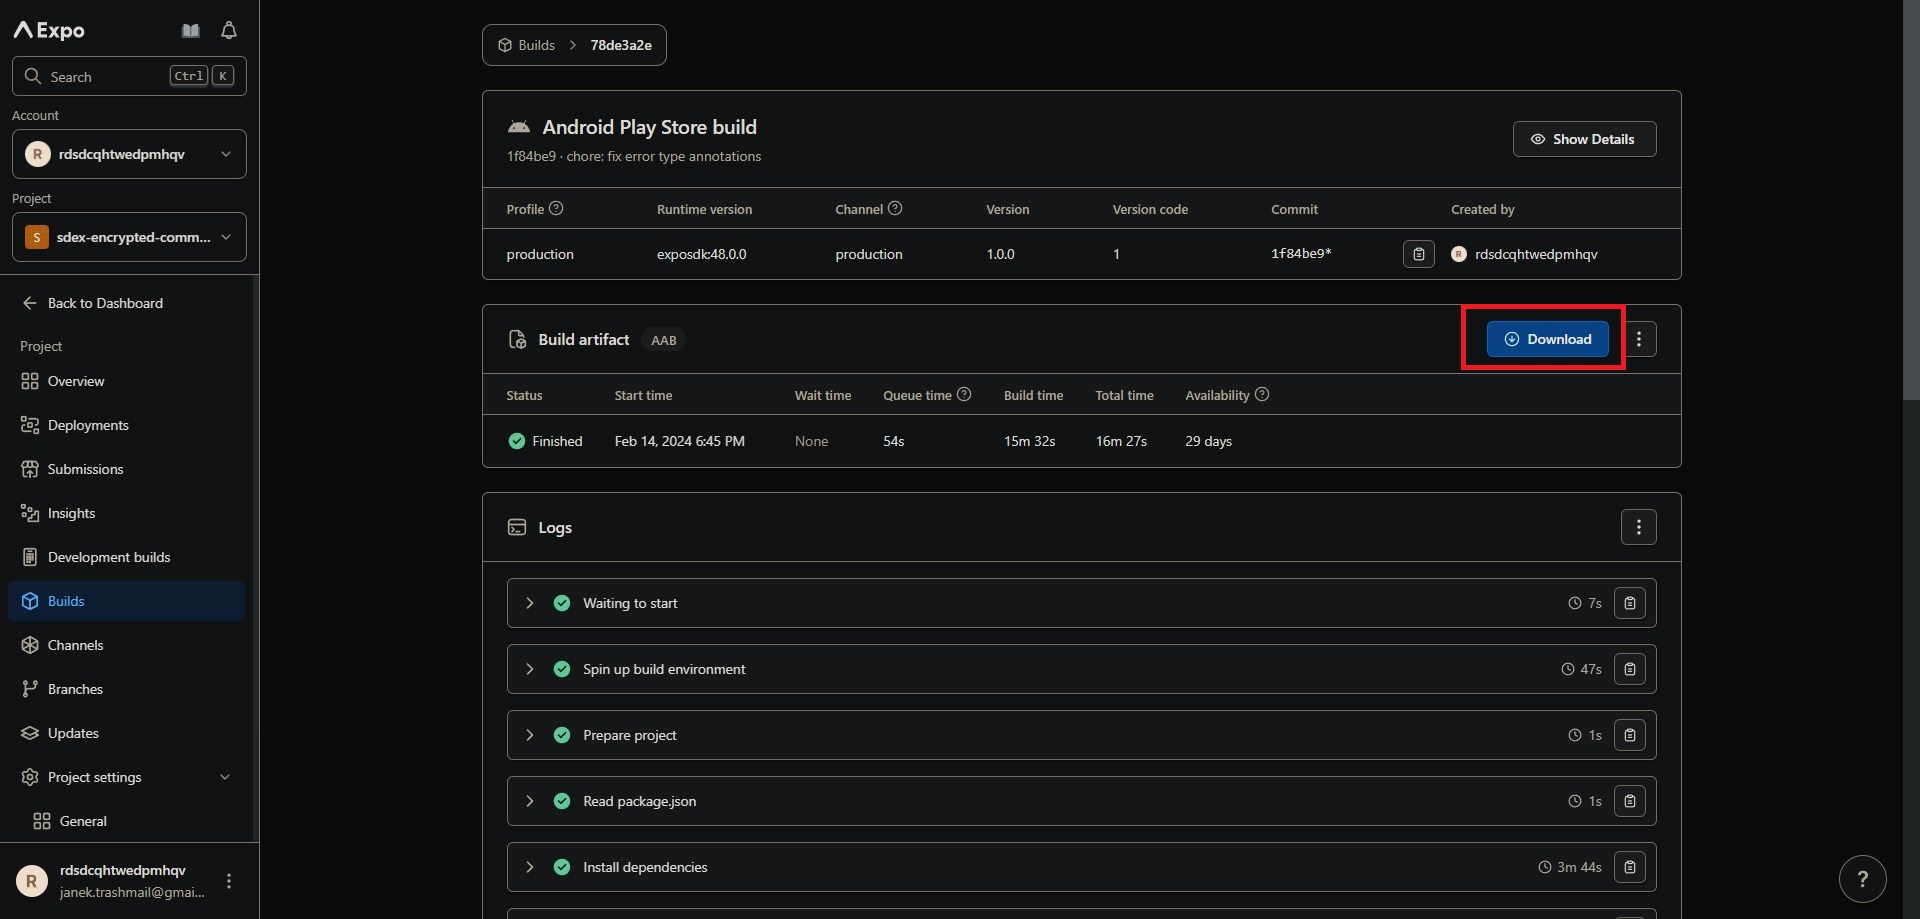
\includegraphics[scale=0.31]{download-apk-2.jpg}
    \captionsetup{justification=centering}
	\caption{Widok strony ze szczegółami wybranej wersji (buildu) aplikacji i linkiem do pobrania}
	\source{opracowanie własne}
	\label{fig:download-build}
\end{figure}

Pobrany tym sposobem plik należy wgrać na swoje urządzenie i wybrać go w menadżerze plików na telefonie. Plik \code{.apk} jest wykonywalny i należy go zainstalować.

Istnieje również możliwość uruchomienia aplikacji w emulatorze. W tym celu należy mieć zainstalowane oprogramowanie Android Studio\cite{android_studio} oraz utworzone urządzenie wirtualne (ang. \textit{Android Virtual Device}, AVD), a także biblioteki wymienione na początku tego paragrafu. Wówczas aplikację mobilną możemy uruchomić w powłoce (znajdując się w katalogu głównym aplikacji mobilnej) poprzez wywołanie komendy:

\begin{lstlisting}[style=BashInputStyle]
    $ npx expo run:android --device <nazwa emulatora>
\end{lstlisting}

\end{document}
